\documentclass{report}
\usepackage[francais]{babel}
\usepackage[utf8]{inputenc}
\usepackage[T1]{fontenc}
\usepackage{float}
\usepackage{amssymb}
\usepackage{stmaryrd}

\usepackage{graphicx}
\usepackage{subfig}

\makeatletter
\newcommand{\Spvek}[2][r]{%
  \gdef\@VORNE{1}
  \left(\hskip-\arraycolsep%
  \begin{array}{#1}\vekSp@lten{#2}\end{array}%
  \hskip-\arraycolsep\right)}

\def\vekSp@lten#1{\xvekSp@lten#1;vekL@stLine;}
\def\vekL@stLine{vekL@stLine}
\def\xvekSp@lten#1;{\def\temp{#1}%
  \ifx\temp\vekL@stLine
  \else
  \ifnum\@VORNE=1\gdef\@VORNE{0}
  \else\@arraycr\fi%
  #1%
  \expandafter\xvekSp@lten
  \fi}
\makeatother

\newcommand{\HRule}{\rule{\linewidth}{0.5mm}}
\bibliographystyle{unsrt}
\begin{document}

\begin{titlepage}

  \begin{center}

    \textsc{\LARGE Rapport}\\[1.5cm]

    \textsc{\Large EPITA}\\[0.5cm]

    \HRule \\[0.4cm]
           { \huge \bfseries Métaheuristiques pour l'optimisation difficile}\\[0.4cm]

           \HRule \\[1.5cm]

           \large
           \emph{Auteurs:}\\
           Loïc \textsc{Bethmont}\\
           Victor \textsc{Lenoir}\\

           \vfill

           % Bottom of the page
           {\large \today}

  \end{center}

\end{titlepage}
%\maketitle
\newpage
\tableofcontents
\newpage

\chapter{Introduction}

Une métaheuristique est un algorithme d'optimisation permettant de
résoudre des problèmes difficiles de manière simple.  Un problème est
dis difficile quand il est inconcevable de parcourir la totalité de
l'espace de solutions pour trouver l'optimum global.


Les métaheuristiques sont des algorithmes très géneraux et avec un
haut niveau d'abstraction et peuvent par conséquent être appliquées sur
un grand nombre de problèmes différents.


Ce sont géneralement des méthodes stochastiques itératives qui tentent
de converger vers un optimum global.


Les métaheuristiques sont très utilisées lorsqu'un problème est trop
complexe pour obtenir une solution analytique ou une autre solution
algorithmique ou lorsqu'une solution alternative est trop coûteuse ou
encore lorsqu'on ne connaît pas de méthodes pour résoudre le problème.

\chapter{Algorithmes}

\section{Recuit simulé}

Le recuit simul\'e est une m\'etaheuristique inspir\'ee de la metallurgie.
La technique de recuit consiste \'a controler le refroidissement des m\'etaux
afin d'obtenir des propri\'et\'es physiques optimales. Il a \'et\'e observ\'e qu'un
refroidissement progressif permettait d'atteindre un niveau d'\'energie plus
satisfaisant que si le m\'etal \'etait refroidi d'un coup.\\\\

Le recuit simul\'e s'inspire donc de ce proc\'ed\'e en introduisant un param\`etre
de temp\'erature $T$ et une fonction \'energie $E$, \'a minimiser. L'algorithme
suit alors les \'etapes suivantes:
\begin{enumerate}
\item Initialisation de la temp\'erature et de la solution initiale.
\item Variation al\'eatoire de la solution.
\item Selon la solution obtenu, deux possibilit\'es:
	\begin{itemize}
		\item La nouvelle solution a une meilleure \'energie que l'ancienne,
			elle est alors accept\'ee.
		\item La nouvelle solution a un moins bon niveau d'\'energie, elle
			est accept\'ee avec une probabilit\'e d\'ependant de la temp\'erature
			actuelle et de la diff\'erence d'\'energie (sp\'ecifiquement
			$e^{-\frac{\Delta E}{T}} $, la r\`egle de Metropolis).
	\end{itemize}
\item Lorsqu'un \'equilibre thermique est atteint, la temp\'erature est
		 diminu\'ee. L'\'equilibre thermique est atteint lorsqu'un nombre fix\'e
		 de perturbations total  ou un nombre inf\'erieur de perturbations
		 accept\'ees est effectu\'e.\\\\
\end{enumerate}

Ainsi, la probabilit\'e d'accepter une modification n'am\'eliorant pas l'\'energie
du syst\`eme diminue avec chaque palier de temp\'erature atteint, des solutions
avec de plus petits \'ecarts d'\'energie \'etant plus facilement accept\'ees.\\\\

Un certain nombre de param\`etres doivent donc \^etre choisis pour l'utilisation
de cette m\'etaheuristique:
\begin{itemize}
	\item La temp\'erature initiale (choisie via un param\`etre $\tau_{0}$, 
	d\'efinissant la probabilit\'e initiale moyenne d'acceptation d'une nouvelle
	solution d\'egradante).
	\item La r\`egle de diminution de tempr\'erature (souvent un pourcentage fixe).
	\item Les coefficients d\'efinissant l'\'equilibre thermique.\\\\
\end{itemize}


%Parle vite fais que c'est une methode qui nous vient de la
%metallurgie, j'y fais reference apres
\subsection{Benchmarks}

Dans chacun des tests, effectu\'es sur le probl\`eme
demand\'e, l'\'equilibre thermique est atteint apres 1000n perturbations ou 12n
perturbations accept\'ees, n \'etant la dimension du probl\`eme, soit 25 dans ce
cas, l'algorithme s'arr\^ete apr\`es 3 paliers de temp\'erature sans
changements. De plus, le g\'en\'erateur de nombres al\'eatoires a \'et\'e
initialis\'e avec une graine fixe, permettant notamment de d\'ebuter avec
la m\`eme solution pour chaque test (voir \ref{depart}).\\\\


\begin{figure}[H]
  \centering
  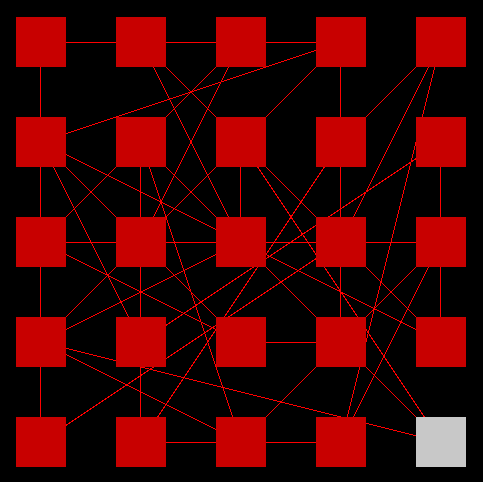
\includegraphics[width=300px]{start.png}
  \caption{La solution de d\'epart, le carr\'e blanc est un bloc bien plac\'e.}
  \label{depart}
\end{figure}

Le choix de param\`etres est tr\`es important pour l'algorithme, comme le montrent
les tableaux suivants.\\\\

\begin{tabular}{|c|c|c|}
 \hline
 $\tau_{0}$ (\%) & It\'erations & \'Energie finale \\
 \hline
 \hline
 10 & 79293  & 200 \\
 \hline
 20 & 78621  & 200 \\
 \hline
 30 & 79298  & 200 \\
 \hline
 40 & 114208 & 280 \\
 \hline
 50 & 114646 & 275 \\
 \hline
 60 & 117261 & 275 \\
 \hline
 70 & 88297  & 200 \\
 \hline
 80 & 100881 & 200 \\
 \hline
 90 & 110317 & 200 \\
 \hline
\end{tabular}


Pour ce premier tableau, des tests ont \'et\'e effectu\'es avec un multiplicateur
de temp\'erature fixe de 0,9. On voit que seuls les valeurs de  $\tau_{0}$ moyennes
ne permettent pas d'atteindre l'optimum. L'algorithme a dans ces cas d\'epass\'e
l'optimum global pour tomber dans un optimum local. Nous avons ensuite fait varier
le multiplicateur pour deux valeurs de  $\tau_{0}$.\\\\

\begin{tabular}{|c|c|c|}
 \hline
 Multiplicateur de temp\'erature & It\'erations & \'Energie finale \\
 \hline
 \hline
0.1 & 13532  & 290 \\
 \hline
0.2  & 16491 & 200 \\
 \hline
0.3  & 18757  & 200 \\
 \hline
0.4  & 22860  & 275 \\
 \hline
0.5  & 23906  & 275 \\
 \hline
0.6  & 27628  & 200 \\
 \hline
0.7  & 37297  & 200 \\
 \hline
0.8  & 54074  & 200 \\
 \hline
0.9  & 110317  & 200 \\
 \hline
\end{tabular}


Ces r\'esultats ont \'et\'e obtenus avec un  $\tau_{0}$ de 0,9, on observe que
faire diminuer le multiplicateur de temp\'erature permet de grandement acc\'elerer
l'algorithme, au prix tout de fois de risquer de tomber dans un minimum local
dans certains cas.\\\\

\begin{tabular}{|c|c|c|}
 \hline
 Multiplicateur de temp\'erature & It\'erations & \'Energie finale \\
 \hline
 \hline
0.1  & 12780  & 330 \\
 \hline
0.2  & 14234  & 260 \\
 \hline
0.3  & 17571  & 280 \\
 \hline
0.4  & 17908  & 200 \\
 \hline
0.5  & 22618  & 265 \\
 \hline
0.6  & 23863  & 200 \\
 \hline
0.7  & 34169  & 200 \\
 \hline
0.8  & 53532  & 270 \\
 \hline
0.9  & 79298  & 200 \\
 \hline
\end{tabular}


Enfin, avec un  $\tau_{0}$ de 0,2, les r\'esultats sont bien moins fiables (le
minimum global n'\'etant atteint que dans 4 cas sur les 9).\\

Ces tests montrent l'importance de ces diff\'erents parem\`etres afin d'atteindre
l'optimum global. Les param\`etres id\'eaux \'etant impossibles \`a pr\'evoir,
il serait int\'eressant dans une application r\'eelle de lancer l'algorithme
plusieurs fois, avec des param\`etres pouvant \^etre diff\'erents afin de
comparer la fr\'equence d'apparition de diff\'erents r\'esultats pour trouver
la solution au probl\`eme (la s\'equence de nombre al\'eatoire \'etant fixe dans
notre cas, les r\'esultats ne d\'ependent plus que des param\`etres, changer la
graine du RNG pourrait aussi permettre de trouver des r\'esultats satisfaisants)\\

\section{Programmation génétique}

Tout comme le recuit simulé, la programmation génétique est une
métaheuristique inspirée d'un autre mécanisme : la sélection
naturelle, expliqué par Charles Darwin.

La sélection naturelle explique l'adaptation des espèces à leur
environnement au fil des génerations. Son principe est simple et
explique que les caractéristiques favorisant la survie/reproduction
d'un individu augmentent en fréquence car l'individu aura plus
tendance à se reproduire/survivre et par conséquent avoir des
descendants et les descendants auront eux aussi cette même
caractéristique favorable à la survie.\\\\

La programmation génétique fonctionne de la même manière, on va
modéliser notre problème de la même manière en utilisant le même
vocabulaire: reproduction, individu, population, séléction.\\\\

La fonction à maximiser/minimiser est appelée fonction de fitness et
indique si un individu "fit"/est adapté à son environnement.\\\\

Le principe de l'algorithme est simple:
\begin{enumerate}
\item Initialisation aléatoire d'une population
\item Reproduction de la population : cross-over, mutation
\item \'Evaluation de fitness pour chaque individu de la population
\item Sélection des individus les plus adaptés (ayant la fitness la plus élevé)
\item Répeter étape 2,3,4 jusqu'à convergence
\end{enumerate}

Il faut noter que même si la programmation génétique est une méthode
de résolution très abstraite, elle nécessite un certain nombre de
paramètres : la taille de la population initial, le nombre de
cross-over/mutation, le nombre d'individus sélectionnés à l'étape 4.
De plus il faut noter que tout comme dans la sélection naturelle, la
mutation est primordiale à l'évolution, en effet elle permet
d'introduire de nouvelles caractéristiques dans une population. Sans
celà on ne ferait que des combinaisons de caractéristiques déjà
existantes.

\subsection{Benchmarks}

Les benchmarks de la programmation génétique ont été réalisé sur des
fonctions à minimiser. Les minimums globaux de cette fonction sont
connus et ainsi on pourra vérifier que le minimum global est
atteint.\\ Ci-dessous la fonction Schwefel de la forme:
$$SH(x) = \sum_{i=1}^{n}{-x_i\sin{(\sqrt{\mid{}x_i\mid{}})}}$$ Un
individu est caracterisé par ses gènes, ici ce sont les $x_i$.  La
figure \ref{geneticschwefel} montre ici l'évolution de la fonction de
Schwefel à 10 variables/gènes au fil des génerations. On observe que
l'algorithme converge bien vers le minimum global connu qui est de
-4189.829.
\begin{figure}[H]
  \centering
  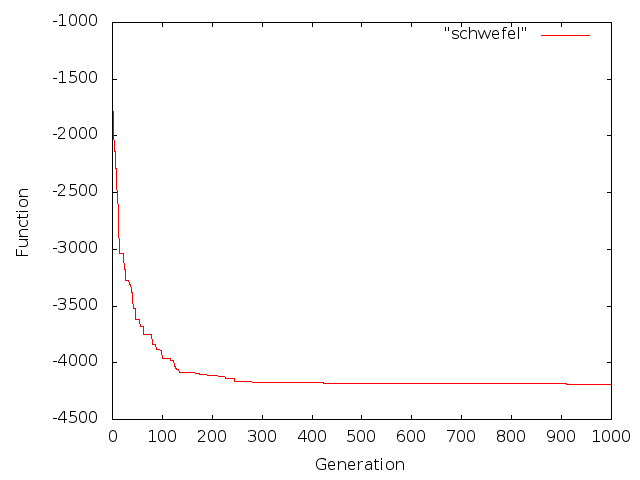
\includegraphics[width=300px]{genetic_schwefel.png}
  \caption{Minimum de la fonction de Schwefel au fil des génerations}
  \label{geneticschwefel}
\end{figure}

On peut observer que la convergence est rapide même si la population
était seulement de 100 individus et que chaque individus avait 10
gènes.

\chapter{Conclusion}

\end{document}
